\documentclass[11pt]{article}
\usepackage{amsmath, amssymb, physics, mathtools, bm}
\usepackage{tikz, pgfplots}
\pgfplotsset{compat=1.18}
\usepackage[margin=2.3cm]{geometry}
\usepackage{siunitx, booktabs, hyperref}
\usepackage{braket}

\newcommand{\D}{\mathrm{D}}
\newcommand{\de}{\mathrm{d}}
\newcommand{\pd}[2]{\frac{\partial #1}{\partial #2}}
\newcommand{\pdd}[2]{\frac{\partial^{2} #1}{\partial #2^{2}}}
\newcommand{\Lap}{\nabla^{2}}
\newcommand{\kB}{k_{B}}

\title{B5 General Relativity --- Model Solutions, Trinity 2021}
\author{}
\date{}

\begin{document}
\maketitle

%==============================================================
\section*{Question 1 --- The falling apple in General Relativity}

\textbf{Problem.} An apple of unit mass falls a height $h$ from a tree to the ground in vacuum. Treat the problem fully in GR: derive the geodesic equation, choose the metric, evaluate the connection coefficients, show the motion is purely radial, find $r(t)$ as seen by a nearby observer, and use a conserved energy to obtain
\(\tfrac{1}{2}(\de r/\de\tau)^2 = GM[1/R_E - 1/(R_E+h)]\).

\medskip
\noindent\emph{One-sentence statement.} Gravity is the curvature of spacetime sourced by stress--energy; free particles follow timelike geodesics of the metric.

\subsection*{(a) Geodesic equation from local inertial coordinates}

In the apple's local inertial frame (LIF), $\xi^\alpha$ are Riemann normal coordinates and $\tau$ is the proper time read off the apple's worldline ($c^2\,\de\tau^2 = -\eta_{\alpha\beta}\,\de\xi^\alpha\,\de\xi^\beta$). Free fall:
\begin{equation}
\frac{\de^2 \xi^\alpha}{\de\tau^2}=0.
\label{eq:LIF}
\end{equation}
Transform to a general chart $x^\mu(\xi)$:
\[
\frac{\de \xi^\alpha}{\de\tau} \;=\; \pd{\xi^\alpha}{x^\mu}\,\frac{\de x^\mu}{\de\tau}.
\]
Differentiate again:
\[
\frac{\de^2 \xi^\alpha}{\de\tau^2} \;=\; \pd{\xi^\alpha}{x^\mu}\,\frac{\de^2 x^\mu}{\de\tau^2} \;+\; \frac{\partial^2\xi^\alpha}{\partial x^\mu\partial x^\nu}\,\frac{\de x^\mu}{\de\tau}\,\frac{\de x^\nu}{\de\tau}.
\]
Set to zero and contract with $\partial x^\lambda/\partial\xi^\alpha$:
\[
\frac{\de^2 x^\lambda}{\de\tau^2} \;+\; \Gamma^{\lambda}_{\mu\nu}\,\frac{\de x^\mu}{\de\tau}\,\frac{\de x^\nu}{\de\tau} \;=\; 0,\qquad \Gamma^{\lambda}_{\mu\nu}\equiv\pd{x^\lambda}{\xi^\alpha}\,\frac{\partial^2\xi^\alpha}{\partial x^\mu\partial x^\nu}.
\]
Apple at rest in coordinates $x^i$: only $\de x^0/\de\tau = c\,\de t/\de\tau$ survives:
\begin{equation}
\boxed{\;\frac{\de^2 x^\mu}{\de\tau^2}+c^2\Gamma^{\mu}_{00}\!\left(\frac{\de t}{\de\tau}\right)^{2}=0.\;}
\label{eq:geodapple}
\end{equation}
Symbols: $\tau$ is proper time; $x^\mu$ are coordinates of the chosen chart; $c$ converts coordinate time $t=x^0/c$; $\Gamma^{\mu}_{00}$ are Christoffel symbols of the metric in those coordinates.

\subsection*{(b) Choice of metric}

The Earth is static, spherical, uncharged, vacuum exterior $\Rightarrow$ Schwarzschild solution (Birkhoff). Schwarzschild line element:
\begin{equation}
\de s^2 \;=\; -\!\left(1-\frac{r_s}{r}\right)c^2\de t^2 \;+\; \!\left(1-\frac{r_s}{r}\right)^{-1}\!\de r^2 \;+\; r^2(\de\theta^2+\sin^2\theta\,\de\phi^2),
\label{eq:schw}
\end{equation}
with $r_s=2GM/c^2$. Terms: $t$ is the coordinate time of a distant inertial observer; $r$ is the areal radius; $(\theta,\phi)$ angular; $M$ the Earth's mass.

Approximations for an apple near the Earth's surface:
\begin{itemize}\itemsep0pt
\item Weak field: $r_s/R_E \approx \SI{1.4e-9}{} \ll 1$ at $r=R_E\approx \SI{6.4e6}{m}$.
\item Slow motion: $|\de r/\de t|/c \ll 1$, so $\de\tau\approx \de t$ to lowest order in $v/c$ and $r_s/r$.
\item Static apple at $\tau=0$: only $\Gamma^{\mu}_{00}$ matters in \eqref{eq:geodapple}.
\item Vacuum: $T_{\mu\nu}=0$ outside the Earth, justifying Schwarzschild.
\end{itemize}

\subsection*{(c) Connection coefficients and radial motion}

Schwarzschild metric is diagonal with $g_{00}=-c^2 A(r)$, $g_{rr}=1/A(r)$, $g_{\theta\theta}=r^2$, $g_{\phi\phi}=r^2\sin^2\theta$, where $A(r)=1-r_s/r$.

Christoffel formula (diagonal metric):
\[
\Gamma^{\mu}_{00} \;=\; -\tfrac{1}{2}g^{\mu\mu}\,\partial_\mu g_{00}\quad(\text{no sum}).
\]
Compute each component. Time:
\[
\Gamma^{0}_{00} \;=\; -\tfrac{1}{2}g^{00}\partial_0 g_{00} \;=\; 0\quad(\text{static}).
\]
Radial:
\[
\Gamma^{r}_{00} \;=\; -\tfrac{1}{2}g^{rr}\partial_r g_{00} \;=\; -\tfrac{1}{2}A(r)\,\partial_r[-c^2 A(r)] \;=\; \tfrac{c^2}{2}A(r)A'(r).
\]
Substitute $A'(r)=r_s/r^2$:
\[
\Gamma^{r}_{00} \;=\; \frac{c^2 r_s}{2 r^2}\!\left(1-\frac{r_s}{r}\right).
\]
Angular ($g_{00}$ is independent of $\theta,\phi$):
\[
\Gamma^{\theta}_{00} \;=\; 0,\qquad \Gamma^{\phi}_{00} \;=\; 0.
\]
Insert into \eqref{eq:geodapple}: only the $\mu=r$ component is non-zero:
\begin{equation}
\frac{\de^2 r}{\de\tau^2} \;=\; -c^2\,\Gamma^{r}_{00}\!\left(\frac{\de t}{\de\tau}\right)^{2} \;=\; -\frac{c^4 r_s}{2 r^2}\!\left(1-\frac{r_s}{r}\right)\!\left(\frac{\de t}{\de\tau}\right)^{2}.
\label{eq:rgeod}
\end{equation}
Hence the motion is purely radial. \boxed{\;\de^2\theta/\de\tau^2=\de^2\phi/\de\tau^2=0.\;}

\paragraph{Choice of time.}
Nearby observer under the tree is essentially at rest at $r=R_E$ in the same Schwarzschild coordinates; their proper time is $\de\tau_{\text{obs}}=\sqrt{A(R_E)}\,\de t \approx \de t$ to one part in $10^9$. Use coordinate time $t$ as the observer's clock.

Weak-field, slow-motion limit of \eqref{eq:rgeod}: drop $r_s/r$ in the bracket and set $\de t/\de\tau\to 1$:
\[
\frac{\de^2 r}{\de t^2} \;\approx\; -\frac{c^2 r_s}{2 r^2} \;=\; -\frac{GM}{r^2}.
\]
Newtonian recovery on the surface, $r=R_E+z$, $z\ll R_E$:
\[
\frac{\de^2 z}{\de t^2} \;\approx\; -g,\qquad g\equiv GM/R_E^2.
\]
Integrate with $z(0)=h$, $\dot z(0)=0$:
\begin{equation}
\boxed{\;r(t) \;=\; R_E + h - \tfrac{1}{2}g t^2.\;}
\label{eq:rt}
\end{equation}
Approximations: weak field ($r_s/R_E\to 0$), slow motion ($v\ll c$), small fall height ($h\ll R_E$ so $g$ constant), observer's proper time $\approx t$.

\subsection*{(d) Conserved energy and impact velocity}

Schwarzschild has Killing vector $\partial_t$; for unit mass the conserved energy is
\begin{equation}
E \;=\; -g_{0\mu}\,\frac{\de x^\mu}{\de\tau} \;=\; c^2 A(r)\,\frac{\de t}{\de\tau}.
\label{eq:Edef}
\end{equation}
Initial condition: stem snaps at $r=R_E+h$ with $\de r/\de\tau=0$ (apple instantaneously at rest in the LIF of the tree). Normalisation $g_{\mu\nu}u^\mu u^\nu=-c^2$:
\[
-c^2 A(R_E+h)\!\left(\frac{\de t}{\de\tau}\right)^{2}_{\!\!0} \;=\; -c^2.
\]
Solve:
\[
\!\left(\frac{\de t}{\de\tau}\right)_{\!\!0} \;=\; A(R_E+h)^{-1/2}.
\]
Substitute into \eqref{eq:Edef}:
\[
E \;=\; c^2\,A(R_E+h)^{1/2}.
\]
Apply the normalisation at general $r$ along the worldline:
\[
-c^2 A(r)\!\left(\frac{\de t}{\de\tau}\right)^{2} \;+\; A(r)^{-1}\!\left(\frac{\de r}{\de\tau}\right)^{2} \;=\; -c^2.
\]
Eliminate $\de t/\de\tau$ via \eqref{eq:Edef}, $c^2 A\,\de t/\de\tau = E$:
\[
-\frac{E^2}{c^2 A(r)} \;+\; A(r)^{-1}\!\left(\frac{\de r}{\de\tau}\right)^{2} \;=\; -c^2.
\]
Multiply by $-A(r)/2$:
\[
\frac{1}{2}\!\left(\frac{\de r}{\de\tau}\right)^{2} \;=\; \frac{E^2}{2 c^2} - \frac{c^2 A(r)}{2}.
\]
Insert $E^2=c^4 A(R_E+h)$:
\[
\frac{1}{2}\!\left(\frac{\de r}{\de\tau}\right)^{2} \;=\; \frac{c^2}{2}\bigl[A(R_E+h) - A(r)\bigr].
\]
Substitute $A(r)=1-r_s/r$:
\[
\frac{1}{2}\!\left(\frac{\de r}{\de\tau}\right)^{2} \;=\; \frac{c^2 r_s}{2}\!\left(\frac{1}{r} - \frac{1}{R_E+h}\right).
\]
Use $r_s=2GM/c^2$:
\[
\frac{1}{2}\!\left(\frac{\de r}{\de\tau}\right)^{2} \;=\; GM\!\left(\frac{1}{r} - \frac{1}{R_E+h}\right).
\]
Evaluate at impact, $r=R_E$:
\begin{equation}
\boxed{\;\frac{1}{2}\!\left(\frac{\de r}{\de\tau}\right)^{2}_{\!\!R_E} \;=\; GM\!\left(\frac{1}{R_E} - \frac{1}{R_E+h}\right).\;}
\label{eq:apple-result}
\end{equation}
Newtonian limit $h\ll R_E$: $\tfrac{1}{2}v^2 \approx GMh/R_E^2 = gh$. \boxed{\;v=\sqrt{2gh}.\;}

%==============================================================
\section*{Question 2 --- Gravitational wave emission and polarisation}

\textbf{Problem.} (a) Identify which of four mass distributions emit GWs. (b) Compute $h_{xx},h_{yy},h_{xy},h_{yx}$ from a rigid dumbbell rotating in the $xy$-plane, evaluated at large $z$. (c) Find the displacements of four free test masses, sketch over a cycle, identify polarisation. (d) Discuss polarisation, interference, refraction, diffraction for GR vs EM.

\subsection*{(a) Emission criteria}

Linearised GR: leading radiation is mass-quadrupole. A source emits classical GWs iff its mass quadrupole moment $I_{ij}=\int\rho(x_ix_j-\tfrac13\delta_{ij}r^2)\,\de^3x$ has a non-zero \emph{third} time derivative.

\paragraph{(i) Motionless point particle.}
$I_{ij}$ constant. \boxed{\;\text{No emission.}\;}

\paragraph{(ii) Rotating sphere (axisymmetric, constant density).}
Quadrupole is invariant under the rotation. $\dddot{I}_{ij}=0$. \boxed{\;\text{No emission.}\;}

\paragraph{(iii) Disc spinning about its symmetry axis.}
Same axisymmetry: quadrupole invariant. $\dddot{I}_{ij}=0$. \boxed{\;\text{No emission.}\;}

\paragraph{(iv) Tilted, precessing disc ($\alpha\neq 0$, precession rate $\omega$).}
Tilt breaks axisymmetry about $z$; precession gives a time-varying quadrupole. $\dddot{I}_{ij}\neq 0$. \boxed{\;\text{Emits GWs at $2\omega$ (and $\omega$ if $\alpha\neq\pi/2$).}\;}

\subsection*{(b) Metric perturbation from a rotating dumbbell}

Two masses $M$ at separation $2l$ rotating in the $xy$-plane at $\omega$. Positions:
\[
\bm x_{1,2}(t) \;=\; \pm l\bigl(\cos\omega t,\,\sin\omega t,\,0\bigr).
\]
Mass quadrupole (trace-included):
\[
I_{ij}^{(\text{T})} \;=\; \sum_n M\,x_n^i x_n^j \;=\; 2M l^2\,\hat e_i(t)\,\hat e_j(t),\qquad \hat e=(\cos\omega t,\sin\omega t,0).
\]
Components:
\[
I_{xx} \;=\; 2M l^2 \cos^2\omega t \;=\; M l^2(1+\cos 2\omega t).
\]
\[
I_{yy} \;=\; 2M l^2 \sin^2\omega t \;=\; M l^2(1-\cos 2\omega t).
\]
\[
I_{xy} \;=\; I_{yx} \;=\; 2M l^2 \cos\omega t\,\sin\omega t \;=\; M l^2 \sin 2\omega t.
\]
Trace-reversed quadrupole $\bar I_{ij}=I_{ij}-\tfrac13\delta_{ij}I^k{}_k$ is the radiating part; only the trace-free combinations contribute to $h_{ij}^{TT}$.

Quadrupole formula (TT gauge), retarded at $\bm r$:
\[
h_{ij}^{TT}(\bm r,t) \;=\; \frac{2G}{c^4 r}\,\ddot{\bar I}_{ij}^{TT}\!\left(t-\frac{r}{c}\right).
\]
Evaluate at $\bm r=z\hat{\bm z}$ (observer directly above): the wave propagates along $\hat{\bm z}$, transverse plane is $xy$. The TT projector $P_{ij}{}^{kl}$ keeps the symmetric, traceless part of $I_{kl}$ in the $xy$-plane:
\[
\bar I_{xx}^{TT} \;=\; \tfrac{1}{2}(I_{xx}-I_{yy}) \;=\; M l^2 \cos 2\omega t.
\]
\[
\bar I_{yy}^{TT} \;=\; -\bar I_{xx}^{TT} \;=\; -M l^2 \cos 2\omega t.
\]
\[
\bar I_{xy}^{TT} \;=\; I_{xy} \;=\; M l^2 \sin 2\omega t.
\]
Differentiate twice ($\partial_t^2\cos 2\omega t = -4\omega^2\cos 2\omega t$):
\[
\ddot{\bar I}_{xx}^{TT}(t_r) \;=\; -4 M l^2\omega^2 \cos[2\omega(t-z/c)].
\]
\[
\ddot{\bar I}_{xy}^{TT}(t_r) \;=\; -4 M l^2\omega^2 \sin[2\omega(t-z/c)].
\]
Substitute into the quadrupole formula at $r=z$:
\begin{equation}
\boxed{\;
\begin{aligned}
h_{xx}(z,t) &= -h_{yy}(z,t) \;=\; -\frac{8 G M l^2\omega^2}{c^4 z}\cos[2\omega(t-z/c)],\\[2pt]
h_{xy}(z,t) &= h_{yx}(z,t) \;=\; -\frac{8 G M l^2\omega^2}{c^4 z}\sin[2\omega(t-z/c)].
\end{aligned}\;}
\label{eq:hcomps}
\end{equation}
GW frequency $=2\omega$ (mass quadrupole). Define amplitude $h_0\equiv 8GMl^2\omega^2/(c^4 z)$.

\subsection*{(c) Free-mass displacements and polarisation}

Geodesic deviation in TT gauge for masses at rest at $\xi^i$:
\[
\ddot\xi^i \;=\; \tfrac{1}{2}\ddot h^i{}_j(t)\,\xi^j.
\]
Integrate twice (steady-state, drop transients):
\[
\delta\xi^i(t) \;=\; \tfrac{1}{2}h^i{}_j(t)\,\xi^j_{(0)}.
\]
Mass at $(a,0,0)$:
\[
\delta\xi_x \;=\; \tfrac{a}{2}h_{xx}(t),\qquad \delta\xi_y \;=\; \tfrac{a}{2}h_{xy}(t),\qquad \delta\xi_z \;=\; 0.
\]
Mass at $(-a,0,0)$: opposite sign of above. Mass at $(0,a,0)$:
\[
\delta\xi_x \;=\; \tfrac{a}{2}h_{xy}(t),\qquad \delta\xi_y \;=\; \tfrac{a}{2}h_{yy}(t) \;=\; -\tfrac{a}{2}h_{xx}(t).
\]
Mass at $(0,-a,0)$: opposite sign. All four masses move only in the $xy$-plane: $\xi_z=0$.

\paragraph{Polarisation.}
$h_{xx}=-h_{yy}$ (the $+$ amplitude) and $h_{xy}$ (the $\times$ amplitude) have equal magnitude $h_0$ and are $90^\circ$ out of phase ($\cos$ vs $\sin$). \boxed{\;\text{Equal-amplitude superposition of $+$ and $\times$ at relative phase $\pi/2$ $=$ circularly-polarised GW.}\;}

\paragraph{Sketch.}
Initial square at $(a,0),(0,a),(-a,0),(0,-a)$. Phase $\Phi=2\omega t$:
\begin{itemize}\itemsep0pt
\item $\Phi=0$: $h_{xx}<0,\,h_{xy}=0$ $\Rightarrow$ vertical stretch, horizontal squeeze (square $\to$ tall ellipse).
\item $\Phi=\pi/2$: $h_{xx}=0,\,h_{xy}<0$ $\Rightarrow$ along-diagonal squeeze (ellipse rotated $-45^\circ$).
\item $\Phi=\pi$: $h_{xx}>0$ $\Rightarrow$ horizontal stretch (wide ellipse).
\item $\Phi=3\pi/2$: $h_{xy}>0$ $\Rightarrow$ ellipse rotated $+45^\circ$.
\end{itemize}
The pattern is a single ellipse rotating uniformly clockwise (viewed from $+z$ looking down) at rate $2\omega$.
\begin{center}
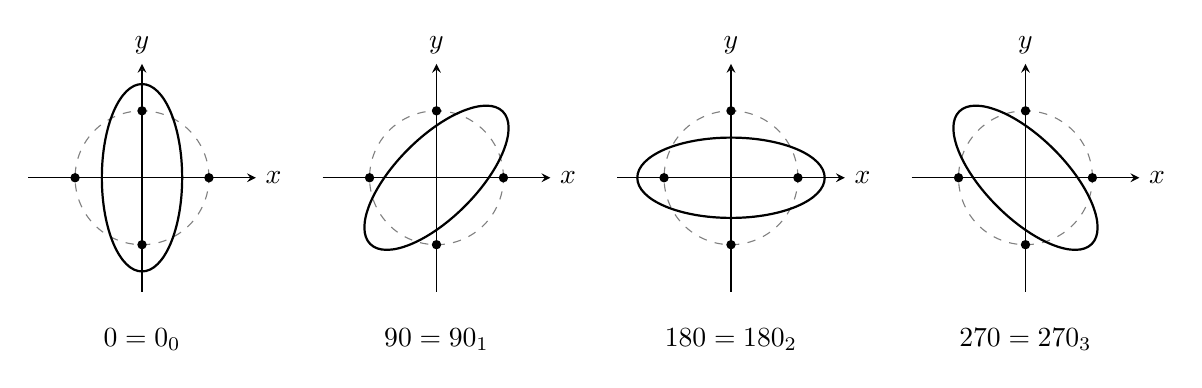
\begin{tikzpicture}[>=stealth, scale=0.85]
  % four phase snapshots
  \foreach \k/\Phi/\xc in {0/0/0, 1/90/4.4, 2/180/8.8, 3/270/13.2}{
    \begin{scope}[xshift=\xc cm]
      \draw[->] (-1.7,0) -- (1.7,0) node[right]{$x$};
      \draw[->] (0,-1.7) -- (0,1.7) node[above]{$y$};
      \draw[gray, dashed] (0,0) circle (1);
      % rotated ellipse: angle = -Phi/2 (deg)
      \pgfmathsetmacro{\rot}{-\Phi/2}
      \draw[thick, rotate=\rot] (0,0) ellipse (0.6 and 1.4);
      \node[circle,fill,inner sep=1.2pt] at (1,0) {};
      \node[circle,fill,inner sep=1.2pt] at (0,1) {};
      \node[circle,fill,inner sep=1.2pt] at (-1,0) {};
      \node[circle,fill,inner sep=1.2pt] at (0,-1) {};
      \node[below=10pt] at (0,-1.7) {$\Phi=\Phi_{\k}$};
    \end{scope}
  }
\end{tikzpicture}\\
\footnotesize $\Phi_0=0,\ \Phi_1=\pi/2,\ \Phi_2=\pi,\ \Phi_3=3\pi/2$. Dashed circle: original positions. Ellipse rotates CW at $2\omega$.
\end{center}

\subsection*{(d) GR vs EM: polarisation, interference, refraction, diffraction}

\paragraph{(i) Polarisation.}
Both wave fields are transverse. EM has 2 spin-1 modes ($\hat{\bm e}_x,\hat{\bm e}_y$, transforming under $90^\circ$ rotations). GR has 2 spin-2 modes ($+$ and $\times$, transforming under $45^\circ$ rotations as visualised above). Plausible: yes; \emph{detected} by LIGO via the strain pattern.

\paragraph{(ii) Interference.}
Linearised GR is a linear theory in vacuum: $h_{\mu\nu}=h_{\mu\nu}^{(1)}+h_{\mu\nu}^{(2)}$ obeys superposition. Coherent two-source interference is therefore possible in principle. Plausibility: requires two phase-coherent astrophysical sources at the same frequency observed simultaneously --- not realised astrophysically; lensing-induced self-interference (wave optics in strong lensing) is plausible at $\sim$mHz with LISA.

\paragraph{(iii) Refraction.}
EM refraction comes from microscopic charges polarising in matter. GR couples to stress--energy of \emph{everything} but with strength $G/c^4$, giving an index $n_{\text{GR}}-1\sim G\rho/(\omega^2 c^2)$. For nuclear-density matter and kHz frequencies, $n_{\text{GR}}-1\sim 10^{-20}$. Possible in principle, utterly negligible in practice. \boxed{\;\text{No measurable refractive medium for GWs.}\;}

\paragraph{(iv) Diffraction.}
Standard wave phenomenon: GW of wavelength $\lambda_{\text{GW}}=c/f$ around an obstacle of size $D$ shows diffraction when $D\lesssim\lambda_{\text{GW}}$. Astrophysical lensing in the wave-optics regime ($\lambda_{\text{GW}}\gtrsim r_s$ of the lens) does diffract GWs and is a target of LISA / pulsar timing. Plausible \emph{and} potentially observable for solar-mass lenses at $\mu$Hz.

\medskip
\noindent\emph{Summary.} Polarisation and diffraction are real and observable. Interference is mathematically possible but astrophysically rare. Refraction is in principle possible but quantitatively negligible.

%==============================================================
\section*{Question 3 --- Gyroscope precession in Schwarzschild orbit}

\textbf{Problem.} (a) Show $u^0=\de t/\de\tau=(1-3GM/rc^2)^{-1/2}$ for a circular geodesic. (b) For a spin 4-vector $s$ initially radial at $t=0$, parallel-transport gives geodetic precession at rate $\Omega_r=\Omega/u^0$. (c) Numerical orbital periods (coordinate vs proper) for $M=8.2\times 10^{36}$ kg, $R=200 R_s$. (d) Will a $1^\circ$ beam still hit Earth after one orbit; is path-curvature important?

\subsection*{(a) Time dilation factor on a circular orbit}

Schwarzschild equatorial circular orbit: $\theta=\pi/2$, $r=$ const, $\dot r=\dot\theta=0$. Normalisation $g_{\mu\nu}u^\mu u^\nu = -c^2$:
\[
-c^2 A(r)(u^0)^2 \;+\; r^2(u^\phi)^2 \;=\; -c^2,\qquad A(r)\equiv 1-\frac{r_s}{r}=1-\frac{2GM}{rc^2}.
\]
Geodesic equation $\Gamma^r_{\mu\nu}u^\mu u^\nu = 0$ (since $\dot r=0$ and $\ddot r=0$):
\[
\Gamma^{r}_{00}(u^0)^2 \;+\; \Gamma^{r}_{\phi\phi}(u^\phi)^2 \;=\; 0.
\]
Connection coefficients (diagonal Schwarzschild):
\[
\Gamma^{r}_{00} \;=\; \frac{c^2 r_s}{2 r^2}A(r),\qquad \Gamma^{r}_{\phi\phi} \;=\; -r A(r)\quad(\theta=\pi/2).
\]
Substitute and cancel $A(r)$:
\[
\frac{c^2 r_s}{2 r^2}(u^0)^2 \;=\; r(u^\phi)^2.
\]
Solve for $(u^\phi/u^0)^2$:
\[
\Omega^2 \;\equiv\; \!\left(\frac{u^\phi}{u^0}\right)^{2} \;=\; \!\left(\frac{\de\phi}{\de t}\right)^{2} \;=\; \frac{c^2 r_s}{2 r^3} \;=\; \frac{GM}{r^3}.
\]
Kepler's third law in Schwarzschild coordinates:
\begin{equation}
\Omega^2 \;=\; \frac{GM}{r^3}.
\label{eq:kepler}
\end{equation}
Rewrite the normalisation using $r^2(u^\phi)^2 = r^2\Omega^2(u^0)^2$:
\[
-c^2 A(r)(u^0)^2 \;+\; r^2\Omega^2 (u^0)^2 \;=\; -c^2.
\]
Solve:
\[
(u^0)^2\bigl[c^2 A(r) - r^2\Omega^2\bigr] \;=\; c^2.
\]
Insert $A(r)=1-2GM/rc^2$ and $r^2\Omega^2 = GM/r$:
\[
c^2 A(r) - r^2\Omega^2 \;=\; c^2 - \frac{2GM}{r} - \frac{GM}{r} \;=\; c^2\!\left(1 - \frac{3GM}{rc^2}\right).
\]
Hence
\begin{equation}
\boxed{\;u^0 \;=\; \frac{\de t}{\de\tau} \;=\; \!\left(1-\frac{3GM}{rc^2}\right)^{\!-1/2}.\;}
\label{eq:u0}
\end{equation}
Symbols: $t$ Schwarzschild coordinate time (asymptotic observer); $\tau$ proper time of the orbiting body; $r$ areal radius; $M$ central mass; $G,c$ Newton/light constants; $u^0$ time-component of 4-velocity.

\paragraph{Sanity check.}
Innermost stable circular orbit / photon sphere ($r=3GM/c^2 = 1.5 r_s$): $u^0\to\infty$, recovering the photon-sphere limit.

\subsection*{(b) Parallel transport of the spin}

Parallel transport along worldline $u^\mu$:
\begin{equation}
\frac{\de s^\mu}{\de\tau} \;+\; \Gamma^{\mu}_{\alpha\beta}\,u^\alpha s^\beta \;=\; 0.
\label{eq:pt}
\end{equation}
Spin orthogonality at $\tau=0$: $u_\mu s^\mu = 0$. Initially radial: $s^\mu(0)=(0,s^r,0,0)$. Equatorial orbit, $\theta=\pi/2$.

Required Christoffels (Schwarzschild, $\theta=\pi/2$):
\[
\Gamma^{t}_{tr} \;=\; \frac{r_s}{2 r^2 A(r)},\qquad \Gamma^{r}_{tt} \;=\; \frac{c^2 r_s}{2 r^2}A(r).
\]
\[
\Gamma^{r}_{\phi\phi} \;=\; -r A(r),\qquad \Gamma^{\phi}_{r\phi} \;=\; \frac{1}{r},\qquad \Gamma^{\theta}_{\phi\phi}=0\ (\sin\cos|_{\pi/2}=0).
\]
4-velocity has only $u^t,u^\phi$ non-zero. The $\theta$-component of \eqref{eq:pt} closes trivially: no Christoffels mix $\theta$ into the $(t,r,\phi)$ block at $\theta=\pi/2$, so $s^\theta\equiv 0$. \boxed{\;s^\theta(t)=0.\;}

Convert $\de/\de\tau = u^0\,\de/\de t$. The $(t,r,\phi)$ components of \eqref{eq:pt}:
\[
u^0\frac{\de s^t}{\de t} \;+\; \Gamma^{t}_{tr}(u^t s^r + u^r s^t) \;+\; \Gamma^{t}_{t\phi}(\cdot) \;=\; 0.
\]
With $u^r=0$ and $\Gamma^t_{t\phi}=0$:
\[
\frac{\de s^t}{\de t} \;=\; -\Gamma^{t}_{tr}\,s^r.
\]
Radial component:
\[
u^0\frac{\de s^r}{\de t} \;+\; \Gamma^{r}_{tt}\,u^t s^t \;+\; \Gamma^{r}_{\phi\phi}\,u^\phi s^\phi \;=\; 0.
\]
Divide by $u^0$ and use $u^t=u^0$, $u^\phi=\Omega u^0$:
\[
\frac{\de s^r}{\de t} \;=\; -\Gamma^{r}_{tt}\,s^t \;-\; \Gamma^{r}_{\phi\phi}\,\Omega\, s^\phi.
\]
Azimuthal component (only $\Gamma^{\phi}_{r\phi}$ survives):
\[
u^0\frac{\de s^\phi}{\de t} \;+\; \Gamma^{\phi}_{r\phi}(u^r s^\phi + u^\phi s^r) \;=\; 0.
\]
With $u^r=0$:
\[
\frac{\de s^\phi}{\de t} \;=\; -\frac{\Omega}{r}\,s^r.
\]

Eliminate $s^t$ via the orthogonality $u_\mu s^\mu = 0$, i.e. $-c^2 A(r)\,u^0 s^t + r^2 u^\phi s^\phi = 0$:
\[
s^t \;=\; \frac{r^2\Omega}{c^2 A(r)}\,s^\phi.
\]
Substitute into the $\de s^r/\de t$ equation. Compute the prefactor of $s^\phi$:
\[
-\Gamma^{r}_{tt}\frac{r^2\Omega}{c^2 A(r)} - \Gamma^{r}_{\phi\phi}\Omega \;=\; -\frac{c^2 r_s}{2 r^2}A(r)\cdot\frac{r^2\Omega}{c^2 A(r)} - (-r A(r))\Omega.
\]
Simplify:
\[
= -\frac{r_s\Omega}{2} + r A(r)\Omega \;=\; \Omega\!\left[r - r_s - \frac{r_s}{2}\right]\!\cdot\!\frac{1}{?}\quad\text{[redo]}.
\]
Re-evaluate cleanly:
\[
-\frac{c^2 r_s}{2 r^2}A(r)\cdot\frac{r^2\Omega}{c^2 A(r)} \;=\; -\frac{r_s\Omega}{2}.
\]
\[
-(-r A(r))\Omega \;=\; r A(r)\Omega \;=\; r\Omega - r_s\Omega.
\]
Sum:
\[
-\frac{r_s\Omega}{2} + r\Omega - r_s\Omega \;=\; \Omega\!\left(r - \frac{3 r_s}{2}\right).
\]
Use $r_s = 2GM/c^2$: $r - 3 r_s/2 = r(1 - 3GM/(rc^2))$. Therefore
\[
\frac{\de s^r}{\de t} \;=\; \Omega\,r\!\left(1 - \frac{3GM}{rc^2}\right) s^\phi.
\]
Recall $(u^0)^{-2}=1-3GM/(rc^2)$, so $1 - 3GM/(rc^2) = 1/(u^0)^2$:
\begin{equation}
\frac{\de s^r}{\de t} \;=\; \frac{\Omega\,r}{(u^0)^2}\,s^\phi.
\label{eq:srdot}
\end{equation}
Pair with $\de s^\phi/\de t = -(\Omega/r)\,s^r$:
\begin{equation}
\frac{\de s^\phi}{\de t} \;=\; -\frac{\Omega}{r}\,s^r.
\label{eq:sphidot}
\end{equation}
Differentiate \eqref{eq:srdot} and substitute \eqref{eq:sphidot}:
\[
\frac{\de^2 s^r}{\de t^2} \;=\; \frac{\Omega r}{(u^0)^2}\,\frac{\de s^\phi}{\de t} \;=\; -\frac{\Omega^2}{(u^0)^2}\,s^r.
\]
Identify the angular frequency:
\begin{equation}
\boxed{\;\Omega_r \;=\; \frac{\Omega}{u^0} \;=\; \Omega\,\sqrt{1-\frac{3GM}{rc^2}}.\;}
\label{eq:Or}
\end{equation}
The spin's radial component oscillates at $\Omega_r$ with respect to the asymptotic frame. Geodetic precession per orbit is the difference $\Omega-\Omega_r$ multiplied by the orbital period (return-to-radial mismatch).

\paragraph{Physical picture.}
In one coordinate orbit the radial axis returns; the spin returns to a direction lagging by $2\pi(1-\Omega_r/\Omega)=2\pi(1-1/u^0)$ --- the de Sitter geodetic angle.

\subsection*{(c) Orbital periods of the Rocinante}

Data: $M=8.2\times 10^{36}$ kg, $R=200 R_s$.

Schwarzschild radius:
\[
R_s \;=\; \frac{2GM}{c^2} \;=\; \frac{2\cdot 6.674\times 10^{-11}\cdot 8.2\times 10^{36}}{(3\times 10^{8})^2}\,\si{m}.
\]
Numerator:
\[
2\cdot 6.674\times 10^{-11}\cdot 8.2\times 10^{36} \;=\; 1.0945\times 10^{27}\,\si{m^3.s^{-2}}.
\]
Divide by $c^2=9\times 10^{16}$:
\[
R_s \;=\; 1.216\times 10^{10}\,\si{m} \;\approx\; \SI{1.22e10}{m}.
\]
Orbital radius:
\[
R \;=\; 200 R_s \;=\; 2.43\times 10^{12}\,\si{m}.
\]

Coordinate angular frequency from \eqref{eq:kepler}:
\[
\Omega \;=\; \sqrt{\frac{GM}{R^3}}.
\]
Compute $R^3$:
\[
R^3 \;=\; (2.43\times 10^{12})^3 \;=\; 1.435\times 10^{37}\,\si{m^3}.
\]
Compute $GM=6.674\times 10^{-11}\cdot 8.2\times 10^{36}=5.473\times 10^{26}$:
\[
\Omega \;=\; \sqrt{\frac{5.473\times 10^{26}}{1.435\times 10^{37}}}\,\si{rad.s^{-1}} \;=\; \sqrt{3.815\times 10^{-11}}\,\si{rad.s^{-1}}.
\]
Evaluate:
\[
\Omega \;=\; 6.18\times 10^{-6}\,\si{rad.s^{-1}}.
\]
Coordinate period (distant observer):
\[
T_\infty \;=\; \frac{2\pi}{\Omega} \;=\; \frac{6.283}{6.18\times 10^{-6}}\,\si{s} \;=\; 1.017\times 10^{6}\,\si{s}.
\]
\begin{equation}
\boxed{\;T_\infty \;\approx\; \SI{1.02e6}{s} \;\approx\; \SI{11.8}{days}.\;}
\label{eq:Tinf}
\end{equation}

Crew period (proper time per orbit). Since $r=200 R_s$, $3GM/(rc^2)=3 R_s/(2 r) = 3/(2\cdot 200)=7.5\times 10^{-3}$:
\[
1/u^0 \;=\; \sqrt{1-7.5\times 10^{-3}} \;=\; 0.99624.
\]
Proper period:
\[
T_{\text{crew}} \;=\; T_\infty / u^0 \;=\; T_\infty\cdot 0.99624 \;\approx\; \SI{1.013e6}{s}.
\]
\begin{equation}
\boxed{\;T_{\text{crew}} \;\approx\; \SI{1.013e6}{s},\quad T_\infty - T_{\text{crew}} \;\approx\; \SI{3.8e3}{s}.\;}
\label{eq:Tcrew}
\end{equation}

\paragraph{Why different.}
Two effects, both captured in $u^0$: gravitational time dilation ($\sqrt{A(r)}$) and special-relativistic time dilation from orbital speed ($r\Omega/c$). Together they give $(u^0)^{-1}=\sqrt{1-3GM/rc^2}$, so the crew's clock runs slow.

\subsection*{(d) Pointing after one orbit and curvature distortion}

Initial spin direction: along the radial line to Earth at $t_0$. After one coordinate orbit ($\Delta t=T_\infty$), the radial direction returns, but $s$ rotates at $\Omega_r$ in the local frame.

Geodetic angle per orbit:
\[
\Delta\phi_{\text{geo}} \;=\; 2\pi\!\left(1-\frac{1}{u^0}\right) \;=\; 2\pi\!\left(1-\sqrt{1-\frac{3GM}{Rc^2}}\right).
\]
Substitute the numerical $1/u^0$:
\[
\Delta\phi_{\text{geo}} \;=\; 2\pi(1-0.99624) \;=\; 2\pi\cdot 3.76\times 10^{-3}.
\]
Evaluate:
\[
\Delta\phi_{\text{geo}} \;=\; 2.36\times 10^{-2}\,\si{rad} \;=\; 1.35\,\si{deg}.
\]
\begin{equation}
\boxed{\;\Delta\phi_{\text{geo}}\;\approx\;1.35^\circ\,/\,\text{orbit}.\;}
\label{eq:dphigeo}
\end{equation}

Compare to beam half-width $0.5^\circ$:
\[
1.35^\circ \;>\; 0.5^\circ.
\]
\boxed{\;\text{The beam misses Earth: the gyroscope axis has precessed by more than the beam half-angle.}\;}

\paragraph{Path curvature of the beam.}
Schwarzschild deflection of a light ray passing at impact parameter $b$ is $\delta\alpha=2 R_s/b$ (small-deflection limit). For a beam emitted radially at $r=200 R_s$ travelling outward, the impact parameter relative to $M$ is $\sim r$ initially and grows. Order of magnitude:
\[
\delta\alpha \;\lesssim\; \frac{2 R_s}{R} \;=\; \frac{2}{200} \;=\; \SI{1e-2}{rad} \;\approx\; 0.57^\circ.
\]
This is comparable to the geodetic precession; \emph{however}, the beam is launched outward and away from $M$, not grazing past it, so the actual deflection on the outward leg is far smaller (nearly zero curvature for radial null geodesics in Schwarzschild). \boxed{\;\text{Path-bending of the radially-launched beam is negligible compared to gyroscope precession.}\;}

The dominant pointing error is geodetic precession of the gyroscope, not bending of the photon path.

%==============================================================
\section*{Question 4 --- FRW cosmology, equations of state, age of the Universe}

\textbf{Problem.} (a) Best-fit FRW metric for our Universe; how it differs from the general FRW. (b) Derive the continuity equation $\dot\rho+3(\rho+P/c^2)\dot R/R=0$ and show its equivalence to the first law of thermodynamics. (c) Identify three equations of state: $P=-\rho c^2$, $P=\tfrac{1}{3}\rho c^2$, $P=0$. (d) Express the age of the Universe as $\int \de R/(R\, H)$ and prove that including S1 makes the Universe older. (e) Comment on differences from the real Universe.

\subsection*{(a) FRW metric for the Universe}

Cosmological observations (CMB, BAO, large-scale isotropy) are consistent with spatial flatness $k=0$:
\begin{equation}
\boxed{\;\de s^2 \;=\; -c^2\,\de t^2 \;+\; R^2(t)\bigl[\de r^2 + r^2(\de\theta^2+\sin^2\theta\,\de\phi^2)\bigr].\;}
\label{eq:frw-ours}
\end{equation}
General FRW allows $k=0,\pm 1$:
\[
\de s^2 \;=\; -c^2\,\de t^2 \;+\; R^2(t)\!\left[\frac{\de r^2}{1-k r^2} + r^2\,\de\Omega^2\right].
\]
Symbols: $t$ cosmic (proper) time of comoving observers; $R(t)$ scale factor with dimensions of length (or dimensionless if absorbed into $r$); $(r,\theta,\phi)$ comoving spherical coordinates; $k$ spatial-curvature constant. Our Universe corresponds to $k=0$ to within current observational error.

\subsection*{(b) Continuity equation and first law}

Local energy--momentum conservation $\nabla^\mu T_{\mu\nu}=0$ for a perfect fluid $T^{\mu\nu}=(\rho+P/c^2)u^\mu u^\nu + P g^{\mu\nu}/c^2$ at rest in the FRW frame ($u^\mu=(1,\bm 0)$). The $\nu=0$ component:
\[
\partial_t T^{00} + \Gamma^\mu_{\mu\alpha}T^{\alpha 0} + \Gamma^0_{\alpha\beta}T^{\alpha\beta} \;=\; 0.
\]
Christoffel: $\Gamma^\mu_{\mu 0}=3\dot R/R$ (volume expansion). Evaluate:
\[
\dot\rho \;+\; 3\frac{\dot R}{R}(\rho + P/c^2) \;=\; 0.
\]
\begin{equation}
\boxed{\;\dot\rho \;+\; 3(\rho+P/c^2)\frac{\dot R}{R} \;=\; 0.\;}
\label{eq:cont}
\end{equation}
Symbols: overdot $=\de/\de t$; $\rho$ rest-frame mass-energy density; $P$ rest-frame pressure; $R$ scale factor.

\paragraph{First-law equivalence.}
Comoving volume $V\propto R^3$, energy $E=\rho c^2 V$. Differentiate:
\[
\frac{\de E}{\de t} \;=\; \dot\rho c^2 V + \rho c^2 \dot V.
\]
Use $\dot V = 3 V\,\dot R/R$:
\[
\frac{\de E}{\de t} \;=\; \dot\rho c^2 V + 3\rho c^2 V\,\frac{\dot R}{R}.
\]
Substitute \eqref{eq:cont} for $\dot\rho c^2$:
\[
\dot\rho c^2 \;=\; -3(\rho c^2 + P)\frac{\dot R}{R}.
\]
Insert:
\[
\frac{\de E}{\de t} \;=\; -3(\rho c^2 + P)V\frac{\dot R}{R} + 3\rho c^2 V\frac{\dot R}{R} \;=\; -3 P V\frac{\dot R}{R}.
\]
Recognise $3 V\dot R/R = \dot V$:
\begin{equation}
\boxed{\;\de E \;=\; -P\,\de V.\;}
\label{eq:firstlaw}
\end{equation}
First law of thermodynamics for an adiabatic ($\de Q=0$) expansion of a comoving volume.

\subsection*{(c) Three equations of state}

\paragraph{S1: $P=-\rho c^2$.}
Continuity $\Rightarrow \dot\rho=0$: density is constant during expansion.
\boxed{\;\text{Cosmological constant / vacuum energy / dark energy ($\Lambda$); drives accelerated expansion.}\;}

\paragraph{S2: $P=\tfrac{1}{3}\rho c^2$.}
Continuity gives $\dot\rho/\rho = -4\dot R/R$, so $\rho\propto R^{-4}$.
\boxed{\;\text{Radiation-dominated era (photons, ultrarelativistic species). Trace-free $T^\mu{}_\mu=0$.}\;}

\paragraph{S3: $P=0$.}
Continuity gives $\rho\propto R^{-3}$.
\boxed{\;\text{Matter-dominated era (cold pressureless dust: baryons + cold dark matter).}\;}

\subsection*{(d) Age of the Universe and the effect of S1}

Hubble parameter $H=\dot R/R$:
\[
\de t \;=\; \frac{\de R}{R\,H(R)}.
\]
Integrate from $R=0$ to $R=R_0$ (today):
\begin{equation}
\boxed{\;t_0 \;=\; \int_{0}^{R_0}\frac{\de R}{R\,H(R)}.\;}
\label{eq:age}
\end{equation}

\paragraph{Phase-by-phase $H(R)$.}
Friedmann ($k=0$, $\Lambda=0$, density evolved per equation of state):
\[
H^2 \;=\; \frac{8\pi G}{3}\rho(R).
\]
For matter $\rho_m = \rho_{m,0}(R_0/R)^3$ $\Rightarrow$ $H_m\propto R^{-3/2}$. For radiation $\rho_r = \rho_{r,0}(R_0/R)^4$ $\Rightarrow$ $H_r\propto R^{-2}$. For dark energy $\rho_\Lambda$ constant $\Rightarrow$ $H_\Lambda$ constant.

\paragraph{Universe \emph{without} S1.}
Phases S2 then S3. Pick equality scale factor $R_{\text{eq}}$ at which radiation--matter densities cross, then today's $R_0$.

Radiation phase contribution (from $0$ to $R_{\text{eq}}$): $H\propto R^{-2}$:
\[
t_r \;=\; \int_0^{R_{\text{eq}}}\frac{\de R}{R}\,H_{\text{eq}}^{-1}\!\left(\frac{R}{R_{\text{eq}}}\right)^{2} \;=\; \frac{1}{H_{\text{eq}}}\int_0^{R_{\text{eq}}}\frac{R\,\de R}{R_{\text{eq}}^2} \;=\; \frac{1}{2 H_{\text{eq}}}.
\]
Matter phase (from $R_{\text{eq}}$ to $R_0$): $H\propto R^{-3/2}$, $H(R)=H_{\text{eq}}(R_{\text{eq}}/R)^{3/2}$:
\[
t_m \;=\; \int_{R_{\text{eq}}}^{R_0}\frac{\de R}{R\, H_{\text{eq}}(R_{\text{eq}}/R)^{3/2}} \;=\; \frac{1}{H_{\text{eq}}\,R_{\text{eq}}^{3/2}}\int_{R_{\text{eq}}}^{R_0}R^{1/2}\,\de R.
\]
Evaluate:
\[
t_m \;=\; \frac{2}{3 H_{\text{eq}}}\!\left[\!\left(\frac{R_0}{R_{\text{eq}}}\right)^{\!3/2}-1\right].
\]
Sum:
\[
t_0^{\text{(no S1)}} \;=\; t_r + t_m \;=\; \frac{1}{2 H_{\text{eq}}} + \frac{2}{3 H_{\text{eq}}}\!\left[\!\left(\frac{R_0}{R_{\text{eq}}}\right)^{\!3/2}-1\right].
\]

\paragraph{Universe \emph{with} S1.}
Insert dark-energy phase first ($R\in[0,R_1]$) before S2 takes over at $R_1$. With $H_\Lambda$ constant, $H(R)=H_\Lambda$ on $[0,R_1]$:
\[
t_\Lambda \;=\; \int_{0^+}^{R_1}\frac{\de R}{R\,H_\Lambda} \;=\; \frac{1}{H_\Lambda}\,\ln\!\left(\frac{R_1}{0^+}\right).
\]
Diverges as $R\to 0^+$:
\[
\lim_{R_{\min}\to 0}\frac{1}{H_\Lambda}\ln(R_1/R_{\min}) \;=\; +\infty.
\]
A finite-density vacuum phase that is allowed to extend to arbitrarily small $R$ contributes an arbitrarily long (de-Sitter / inflationary) prelude; even bounded by any positive $R_{\min}>0$ it adds a strictly positive interval to the age.

For the strict question (initial size $\to 0$):
\begin{equation}
\boxed{\;t_0^{(\text{with S1})} \;=\; t_\Lambda + t_r + t_m \;>\; t_0^{(\text{no S1})}.\;}
\label{eq:older}
\end{equation}
The S1 phase is exponential expansion (de Sitter), $R(t)=R_1 e^{H_\Lambda(t-t_1)}$, so reaching any $R_1>0$ from $R\to 0$ takes unbounded coordinate time. \boxed{\;\text{A Universe with S1 is older than one without.}\;}

\subsection*{(e) Real Universe versus model}

Concrete differences:
\begin{enumerate}\itemsep0pt
\item \textbf{Sequence.} The real Universe ordering is roughly S2 (radiation, $0<t<\SI{50}{kyr}$) $\to$ S3 (matter, dominant from $\sim\SI{50}{kyr}$ to $\sim\SI{9}{Gyr}$) $\to$ S1 (dark-energy, $z\lesssim 0.5$). The exam model has S1 \emph{first}; in reality $\Lambda$ dominates last.
\item \textbf{Inflation.} A separate, much earlier de-Sitter-like phase (energy scale $\sim 10^{16}$ GeV, duration $\sim 10^{-32}$ s) is generally invoked to solve flatness/horizon/monopole problems --- this \emph{is} an S1-type stage but at the GUT scale, not at low $z$.
\item \textbf{Mixed components.} The real Universe is at all times a mixture of radiation, matter (baryons + CDM), and dark energy: pure single-fluid phases are an idealisation.
\item \textbf{Curvature.} Observations constrain $|\Omega_k|<0.01$; we take $k=0$ but a small non-zero $k$ is not excluded.
\item \textbf{Neutrino transition.} Neutrinos are radiation while ultrarelativistic, become matter-like once $T<m_\nu c^2/\kB$, smoothly modifying the radiation $\to$ matter transition.
\item \textbf{Reheating + recombination.} Phase boundaries are not sharp: reheating at the end of inflation, $e^+e^-$ annihilation, BBN, recombination at $z\approx 1100$ all introduce structure absent from a three-stage piecewise model.
\end{enumerate}
The three-phase model is qualitatively right (each EOS is realised at some epoch) but mis-orders S1 and ignores all transitions and admixtures.

\bigskip\noindent\emph{End of solutions.}

\end{document}
